\documentclass[11pt,english,british]{report}
\usepackage[a4paper]{geometry}
%\usepackage[T1]{fontenc}
\usepackage[latin9]{inputenc}
\usepackage{setspace}

\geometry{verbose,tmargin=3cm,bmargin=3cm,lmargin=3.5cm,rmargin=2.4cm}
\usepackage{amsmath}
\usepackage{amssymb}
\usepackage{cancel}
%\usepackage{gensymb}
\usepackage{graphicx}
\usepackage{esint}
\usepackage{mdsymbol}
\usepackage{esvect} 
%\usepackage{lipsum}
\usepackage{hhline}
\usepackage{eurosym}
\usepackage{listings}
\usepackage{booktabs}
\usepackage{amssymb}
\usepackage{mathrsfs}
\usepackage{commath}
\usepackage{adjustbox}
\usepackage{booktabs}
\usepackage{array}
\usepackage{lscape}
\usepackage[xspace]{ellipsis}
\usepackage{color}
\usepackage{float}
\usepackage{caption}
\usepackage{afterpage}


\definecolor{mygreen}{rgb}{0,0.6,0}
\definecolor{mygray}{rgb}{0.5,0.5,0.5}
\definecolor{mymauve}{rgb}{0.58,0,0.82}
\begin{document}

\title{Placeholder Tex Doc}
\author{Conor Dooley}
\maketitle
\chapter{Background Review}
\section{Brief Overview}
\doublespacing
In a world where the demand for high performance hand-held computing devices continues to grow and the prevalence of ``smart'' devices is increasing the problem of maintaining the steady gain in performance of Systems-On-Chip remains at the forefront. %TODO cite?
The main drivers of performance in Systems-On-Chip are the number of transistors on a chip, the clocking frequency and parallelism. However the latter will not be addressed in this assessment, partly as the performance of the paralellised operation is largely governed by the number of transistors and clock frequency to begin with. %TODO Excessive?
As the number of transistors on a chip has increased roughly following Moore's Law the increase in clock frequency has not been able to follow a similar linear trajectory, which clock frequency having remained roughly equivalent for the last 10 years \cite{ross2008cpu}.

This plateauing of clock frequency has been caused by the high power consumption due to the demands placed by the global distribution of a high frequency clock, which is often the single biggest consumer of power on the chip. %TODO cite (can use tiwari1998reducing)
In a world where low power devices are desirable, especially with the growing demand of Internet-Of-Things where high power consumption goes directly against one of the key pillars of the technology. %TODO Pillars of what?

In digital systems two main approaches are used when designing the clocking system. In both cases the chip is broken down into small areas in which all transistors are clocked synchronously, with the size constrained by the ability to deliver a quality clock signal to all transistors. The first of these methods is Globally Synchronous Locally Synchronous, or GSLS, where all of these sub areas on the chip operate synchronously with each other. In practice however this is very difficult to achieve as extremely high precision is required across the entire area of the chip, and doing so leads to high power consumption.
In contrast a Globally Asynchronous Locally Synchronous clock delivery system ensures that in each sub division of the chip clocking is synchronous however the ``local'' areas are independent from each other. This reduces the clocking system's complexity and thus the power consumption and chip area used at the expense of communication speed between blocks. %TODO citation?
A GSLS system however has the advantages of deterministic behaviour and greater rates of communication between clocking areas and as such remains a desirable system design. A number of methods which deliver GSLS clocking exist at present such as clock trees as well as emerging technologies such as ADPLL networks.

\section{The Impact of Clocking Errors}

In Figure \ref{fig:eldar_why_precise_clocking} the data path between two synchronously clocked registers is shown, with the circuit's function being carried out by the combinatorial network between the registers.
Each register has a setup time, which represents the amount of time that the input value to a register must remain constant before the clock edge, and a hold time, the time for which the input must remain constant after a clock edge.
\begin{figure}[h]
	\centering
	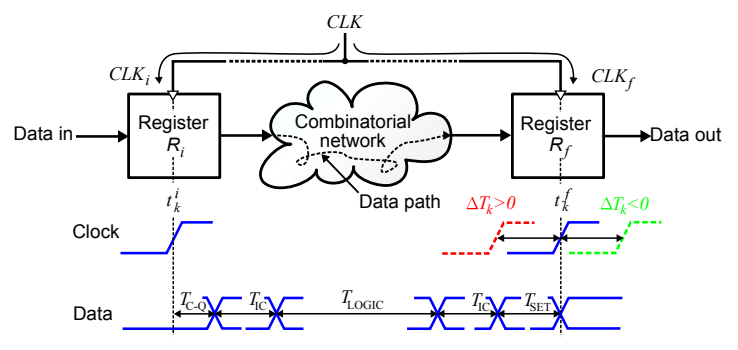
\includegraphics[scale=0.5]{../eldar_why_precise_clocking}
	\caption{Data Flow in a Clocked System \cite{zianbetov2013distributed}.}
	\label{fig:eldar_why_precise_clocking}
\end{figure}\newline
A lack of synchronisation between the clock edges will manifest itself as a time difference between the clocking events at both registers, $\Delta T = t^i_k - t^f_k$. $\Delta T$ is considered to be ergodic and can be described by an average deviation called skew and random process that is normally modelled as a Gaussian random variable. If $\Delta T$ is negative this reduces the time available for the intervening combinatorial network thereby having the same effect as a reduction in clocking frequency.
The most common sources of clock error are caused by mismatches which usually stem from production such as differences in the length of clocking paths, buffer delays or in the parameters of either active or passive components in the clock distribution network. These all manifest themselves as skew, while the noise in active components will appear as jitter in the clock signal.

\section{Traditional Solutions}

A number of traditional solutions exist which provide GSLS clocking systems, using a variety of techniques. The most simple of these use the clock distribution network's symmetry in order to deliver the clock in phase at all locations in the chip and are named according to their geometry with the main variants being branch-trees, X-trees or H-trees. %TODO insert figure
\begin{figure}[h]
	\centering
	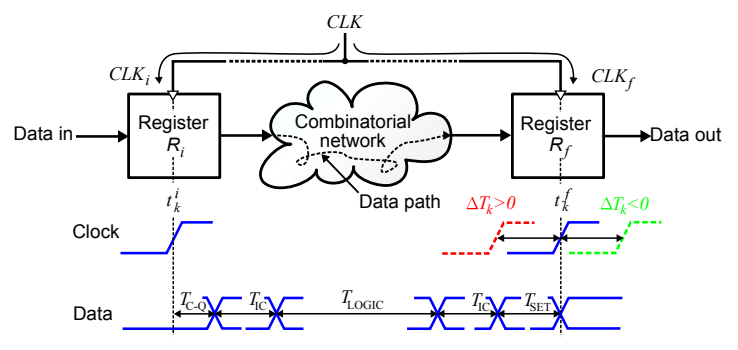
\includegraphics[scale=0.5]{../eldar_why_precise_clocking}
	\caption{Data Flow in a Clocked System \cite{zianbetov2013distributed}.}%TODO insert figure
	\label{fig:trees}
\end{figure}
While on the surface these appear simple the task of obtaining an exact matching is, in practise, the limiting factor in this design. Even if the clock distribution system is geometrically symmetrical production mismatches in either active or passive components will lead to a skew that varies from part to part. In order to minimise the impact of production tolerances the dimensions of components in the distribution network can be increased, thus reducing the relative variation possible. However this has the impact of increasing the power consumption of the distribution network \cite{tiwari1998reducing}.

Designs do exist in which the electrical lines used in the tree network are replaced by waveguides for optical signals, which negates the electrical losses however this technique suffers from being a newer technology and as such is expensive to realise \cite{haurylau2006chip}.

A mesh clock distribution network is an alternate design where the clock is delivered using a Cartesian grid of distribution lines and variation in skew is inversely proportional to the density of the grid. According to Abdelhadi \textit{et al} (2010) clock meshes ``\textit{achieve low and deterministic skew, low skew variations, and low jitter}'', all desirable characteristics for a clock distribution system. However they dissipate more power due to extra capacitive loading due to vast number of lines required to form the grid and similarly to tree distribution networks suffer from potential mismatch in production and alleviation through increasing dimensions will again lead to higher power consumption \cite{abdelhadi2010timing}. 
\begin{figure}[h]
	\centering
	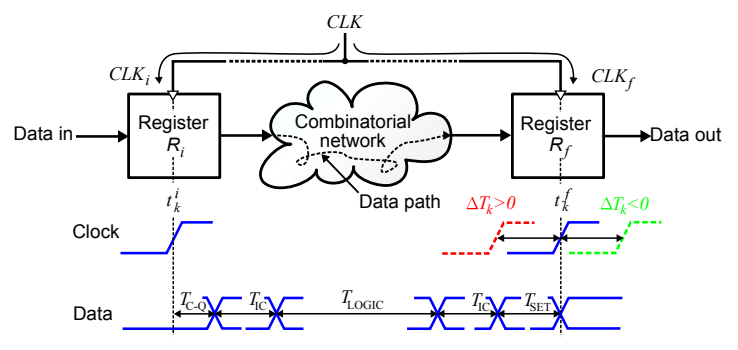
\includegraphics[scale=0.5]{../eldar_why_precise_clocking}
	\caption{Data Flow in a Clocked System \cite{zianbetov2013distributed}.}%TODO insert figure
	\label{fig:mesh}
\end{figure}

In a clocking distribution system using a tree type network the skew due to the manufacturing process can be partly accounted for by means of a skew compensation system, of which there are two main types. These types are defined by the location of the control mechanism with those having one controller located at the clock source being known as ``centralised'' methods and those with multiple controllers in the individual clocking areas known as ``decentralised''. In a centralised skew compensation circuit the skew across the chip is calculated by the central controller which then manipulates the distribution network in order to deliver a more in-phase clock around the chip. This however adds complication to a circuit which already is a large consumer of power and as such increases the power usage.
As the name suggest a decentralised skew compensation technique delegates this responsibility to the individual clock regions. For example Yamashita \textit{et al} designed a system in which each clocking area or ``leaf node'' contains a partial clock tree. Each of these ``leaves'' is able to compare its clock phase to the neighbouring node and based on the result tune an adjustable delay buffer \cite{yamashita2005dynamic}. While this method can compensate for process, voltage and temperature variation it does not address the power consumption due to the delivery of a high frequency clock across the entire chip area.

\section{Multi-oscillator Designs}
The designs described previously are all similar in that they have a single central oscillator that provides the clock for all areas of the chip, whereas the following methods attempt to synchronise multiple oscillators, each of which provides the clock for a single clocking area. The main advantage of a multi-oscillator design is that as each clocking area has its clock created locally there is no problem with signal degradation. Similar to a decentralised skew compensation scheme comparisons are only made to neighbouring blocks and as such there is reduced power loss due to transmission.
\begin{figure}[h]
	\centering
	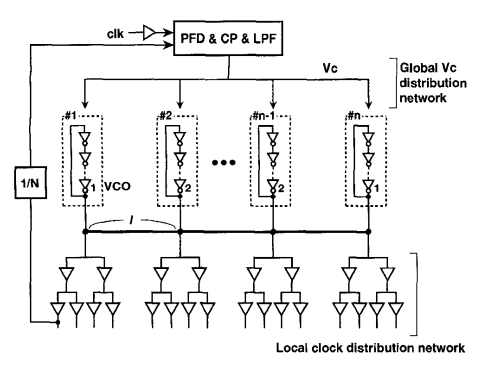
\includegraphics[scale=0.5]{../mizuno1998noise}
	\caption{Coupled Oscillator Clock Delivery Circuit \cite{mizuno1998noise}.}
	\label{fig:mizuno1998noise}
\end{figure}
One such method is a network of oscillators as in Figure \ref{fig:mizuno1998noise} which uses coupled PLLs to generate local clocks. The advantage of this method is that only the control voltage $v_c$ needs delivery to all areas of the chip thus alleviating the need for a power hungry distribution circuit while also being more noise immune than the transmission of a high frequency clock. However this design still suffers from clock variation as all VCOs are fed the same control voltage, and this is acknowledged by the authors:
\begin{quotation}
	\singlespacing
	\textit{Unfortunately, as with the conventional ... method, distributing the VCOs over the entire chip causes the problem that jitter and skew are increased by variations in the fabrication process (static), temperature, and power supply (dynamic)} \cite{mizuno1998noise}.
	\doublespacing
\end{quotation}
This design also only compares the phase of a single branch of the distribution network with the reference in order calculate the control voltage which again may contribute to a degradation in clock synchronisation. %TODO why

Another potential multi-oscillator design synchronises the oscillators using the phase relationship with the oscillators in the neighbouring clocking area. Once again this negates the requirement for a global distribution structure and comparisons need only be made with neighbouring areas, and as a phase lock loop is being used only a divided down version of the clock is required. This in turn means the hardware transporting the divided clock signal to the phase comparator has significantly lower requirements placed on it thus lowering the power consumption. Pratt and Nguyen initially proposed this design in their paper published in 1995 entitled ``\textit{Distributed Synchronous Clocking}'' in which they propose a Cartesian grid of clocking areas, each with their own PLL, which has become known as a PLL Network \cite{pratt1995distributed}. In this design any given node is synchronised with its neighbours and one of the corner nodes is additionally synchronised with the reference. According to the authors this is ``a simple, effective way to achieve low cost, high quality, low skew clock generation in a synchronous parallel processor''. This methodology was implemented by Gutnik \textit{et al} (2000) who found:
\begin{quote}
	\singlespacing
	\textit{Design and measurements on this chip confirm that generating and synchronizing multiple clocks on chip is feasible. Neither the power nor the area overhead of multiple PLLs is substantial compared to the cost of distributing the clock by conventional means} \cite{gutnik2000active}.
	\doublespacing
\end{quote}
\begin{figure}[h]
	\centering
	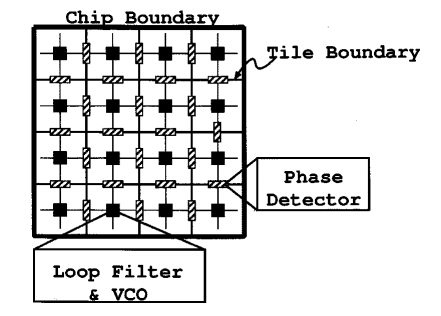
\includegraphics[scale=0.5]{../gutnik2000active}
	\caption{PLL Network Topology \cite{gutnik2000active}.}
	\label{fig:gutnik2000active}
\end{figure}

\section{ADPLL Networks}







\chapter{Progress to Date}



\newpage
\bibliography{bib} 
\bibliographystyle{IEEEtran}

\end{document}
